\documentclass[conference]{IEEEtran}

\usepackage{graphicx}
\usepackage{booktabs}
\usepackage{amsmath}
\usepackage{amssymb}

\title{
Residual-Risk-Guided Discovery of
Stochastic Mixed-Order Capability Interactions
}

\author{
\IEEEauthorblockN{Anonymous Author(s)}
\IEEEauthorblockA{Anonymous Submission}
}

\begin{document}

\maketitle

\begin{abstract}
This is a compilation smoke test for the SCIF v0.0.4 manuscript.
The final abstract and manuscript content will be inserted after the
IEEEtran toolchain has been verified.
\end{abstract}

\section{Introduction}

Combinatorial testing provides a foundation for studying faults caused
by parameter interactions~\cite{kuhn2008beyond}.

This document verifies the IEEE conference template, bibliography, and
publication figure pipeline before conversion of the complete
manuscript.

\begin{figure}[t]
    \centering
    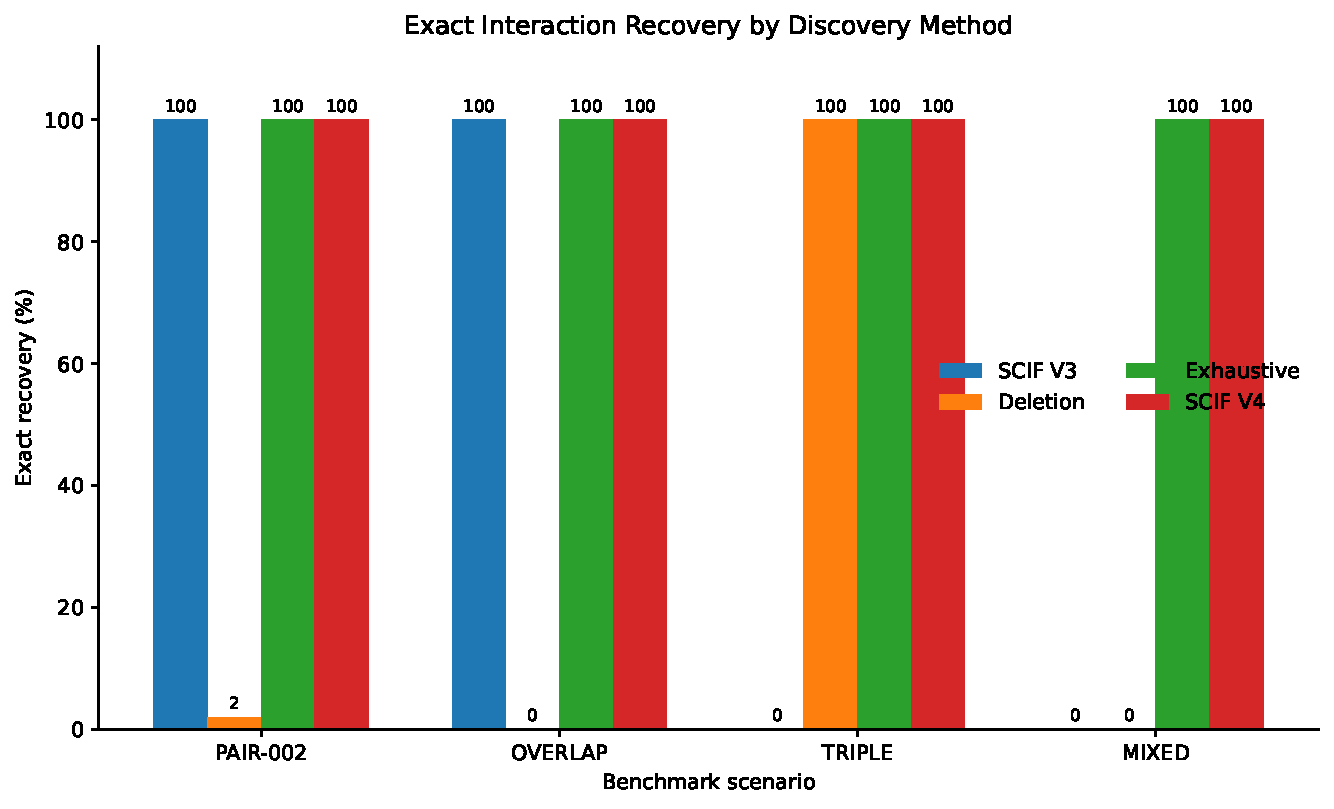
\includegraphics[
        width=\columnwidth
    ]{figures/figure_1_recovery_comparison.pdf}
    \caption{
        Smoke-test rendering of the SCIF method-comparison figure.
    }
    \label{fig:smoke}
\end{figure}

\bibliographystyle{IEEEtran}
\bibliography{references}

\end{document}
